\documentclass[11pt]{article}
\usepackage{graphicx}
\usepackage{float}
\usepackage{hyperref}
\usepackage{natbib}
\usepackage{listings}
\usepackage{xcolor}
\usepackage[dvipsnames]{xcolor}
\usepackage[svgnames]{xcolor}

\setlength{\textwidth}{6.5in}
\setlength{\headheight}{0in}
\setlength{\textheight}{8.0in}
\setlength{\hoffset}{0in}
\setlength{\voffset}{0in}
\setlength{\oddsidemargin}{0in}
\setlength{\evensidemargin}{0in}


\lstdefinestyle{txtstyle}{
    basicstyle=\ttfamily\small,
    breaklines=true,
    backgroundcolor=\color{Bisque}
}
\lstset{style = txtstyle}

\definecolor{codegreen}{rgb}{0,0.6,0}
\definecolor{codegray}{rgb}{0.5,0.5,0.5}
\definecolor{codepurple}{rgb}{0.58,0,0.82}
\definecolor{backcolour}{rgb}{0.95,0.95,0.92}

\lstdefinestyle{mystyle}{
    backgroundcolor=\color{backcolour},   
    commentstyle=\color{codegreen},
    keywordstyle=\color{magenta},
    numberstyle=\tiny\color{codegray},
    stringstyle=\color{codepurple},
    basicstyle=\ttfamily\footnotesize,
    breakatwhitespace=false,         
    breaklines=true,                 
    captionpos=b,                    
    keepspaces=true,                                   
    numbersep=5pt,                  
    showspaces=false,                
    showstringspaces=false,
    showtabs=false,                  
    tabsize=2
}

\title{Computational Physics ps-2 Report}
  
\author{Tongzhou Wang, GitHub account: TZW56203, repository: phys-ga2000}
\date{September 17, 2024}

\begin{document}

\maketitle

\section{Problem 1}
\lstinputlisting[]{codes/ps-2-1_output.txt}

\section{Problem 2}
\lstinputlisting[]{codes/ps-2-2_output.txt}

The following codes were used to compute the minimum and maximum (positive) numbers in \texttt{np.float32} and \texttt{np.float64}.

\lstset{style = mystyle}
\begin{lstlisting}[language=Python]
min32 = np.float32((0 + np.exp2(-23)) * np.exp2(-126))
max32 = np.float32((1 + (1 - np.exp2(-23))) * np.exp2(127))
min64 = np.float64((0 + np.exp2(-52)) * np.exp2(-1022))
max64 = np.float64((1 + (1 - np.exp2(-52))) * np.exp2(1023))
\end{lstlisting}

\section{Problem 3}
\lstset{style = txtstyle}
\lstinputlisting[]{codes/ps-2-3_output.txt}

According to wikipedia, the Madelung constant for a sodium ion in sodium chloride is -1.747565. Here, I only considered L = 50 atoms in each of the three directions. For larger L, the result should approach the true value.

\section{Problem 4}
\begin{figure}[H]
    \centering
    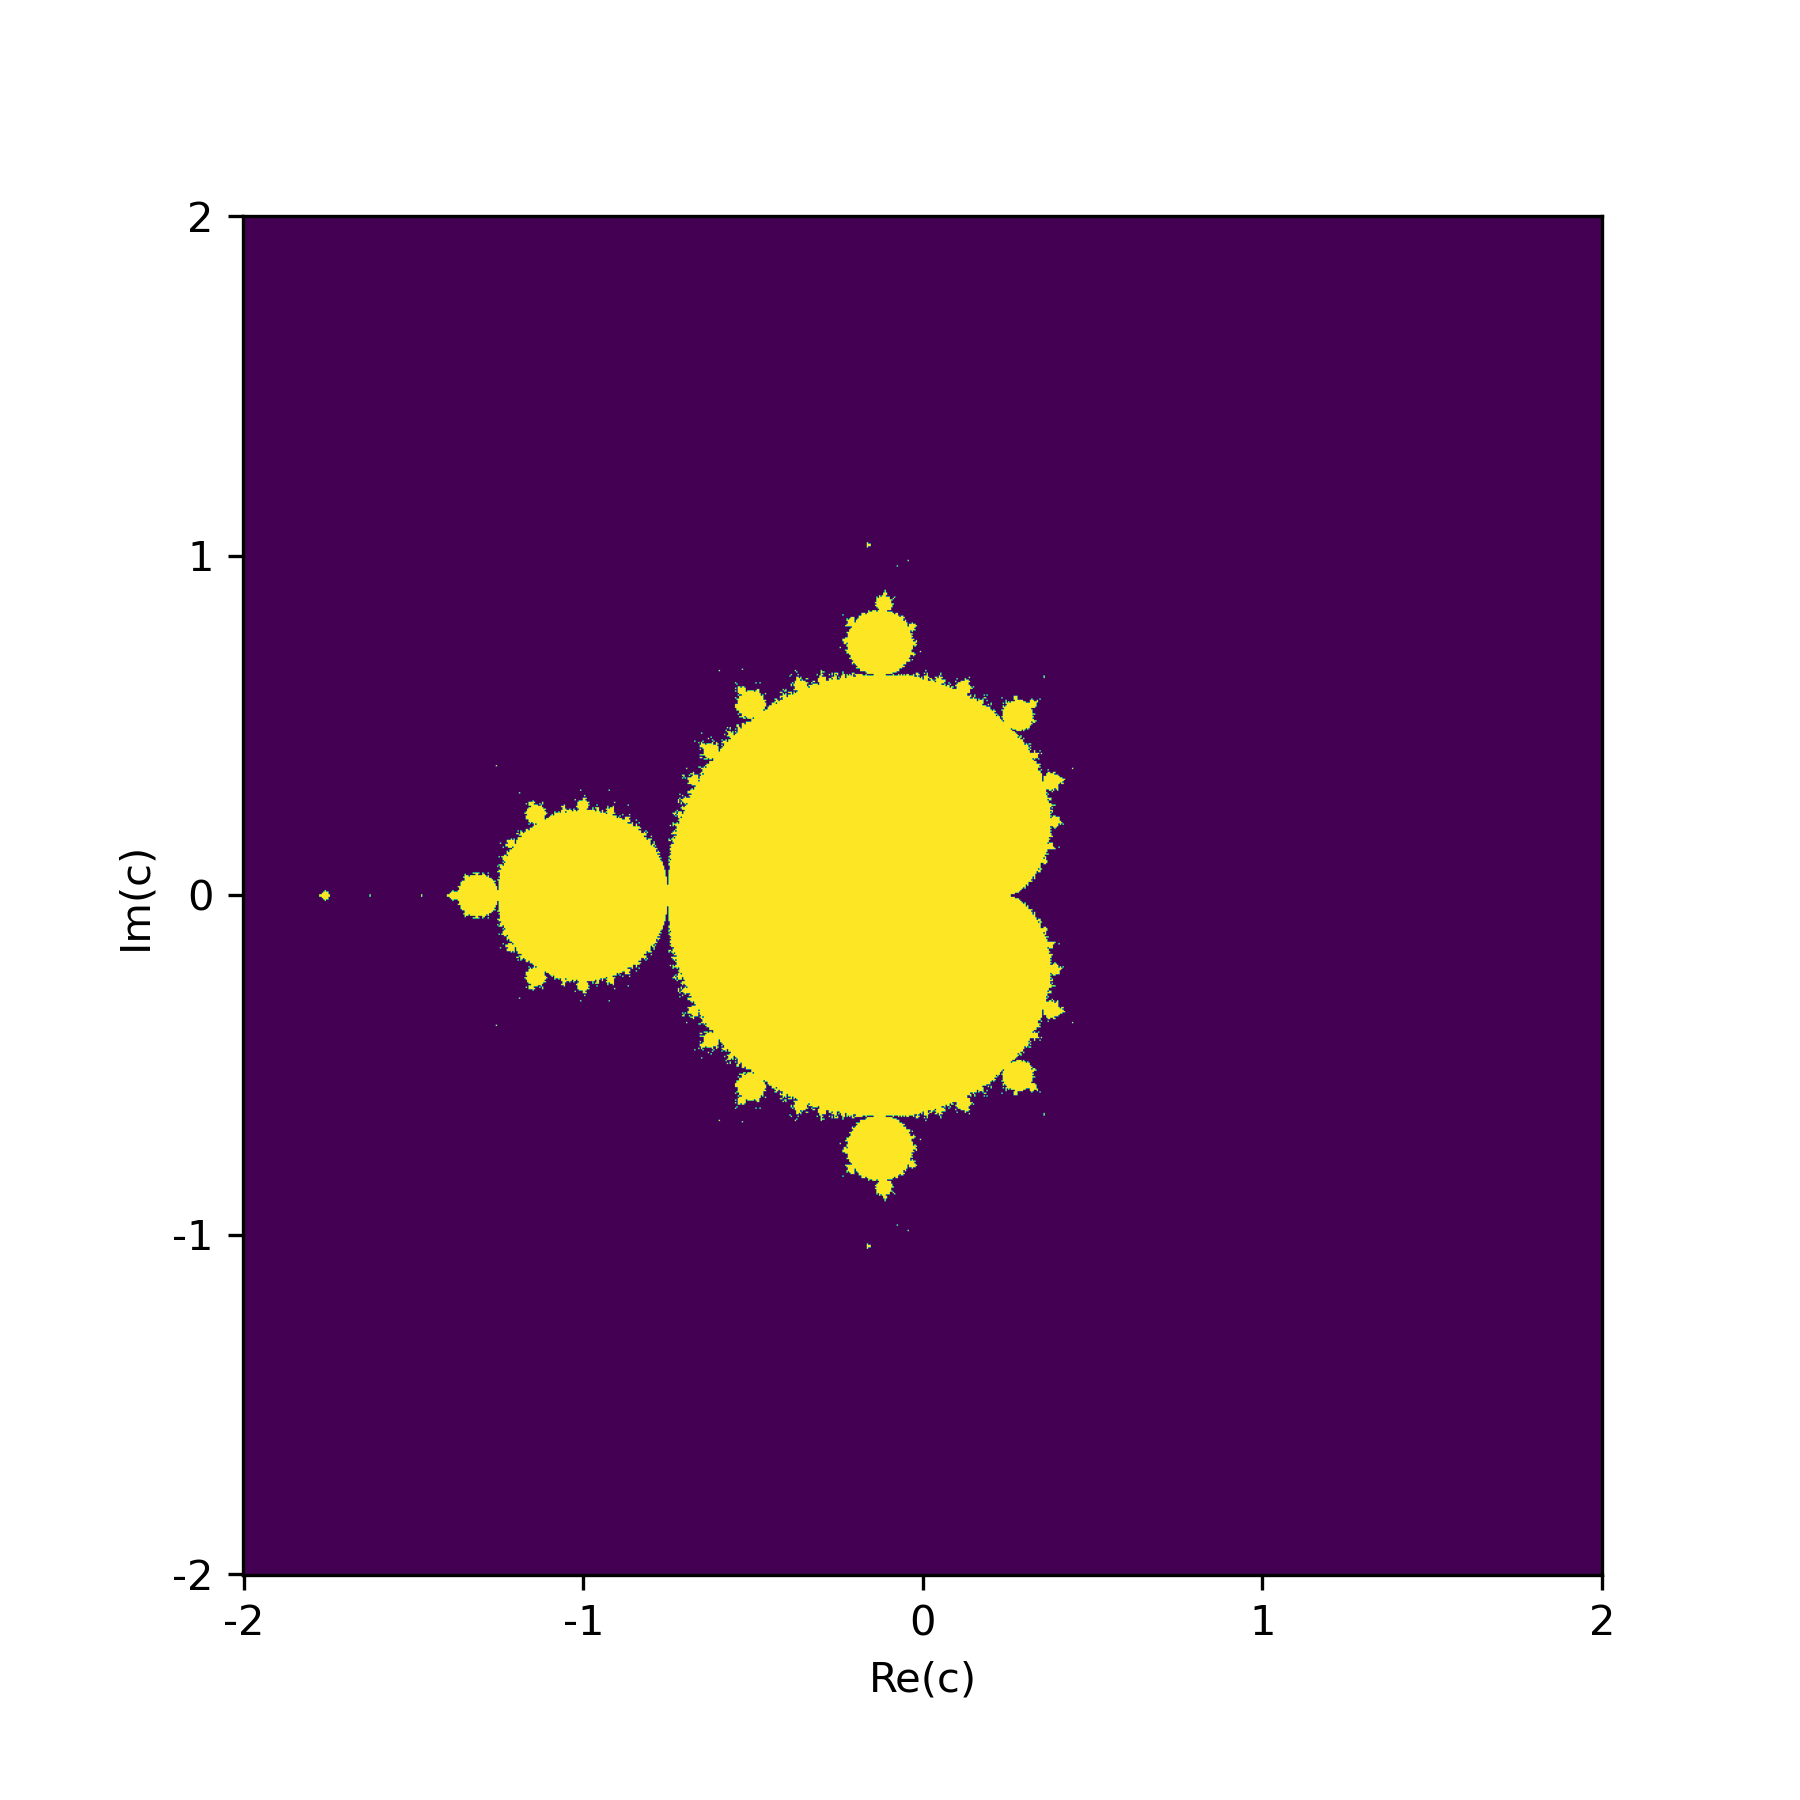
\includegraphics[scale = 0.8]{images/Mandelbrot-set.png}
    \caption{Mandelbrot set.}
\end{figure}

\section{Problem 5}
\begin{figure}[H]
    \centering
    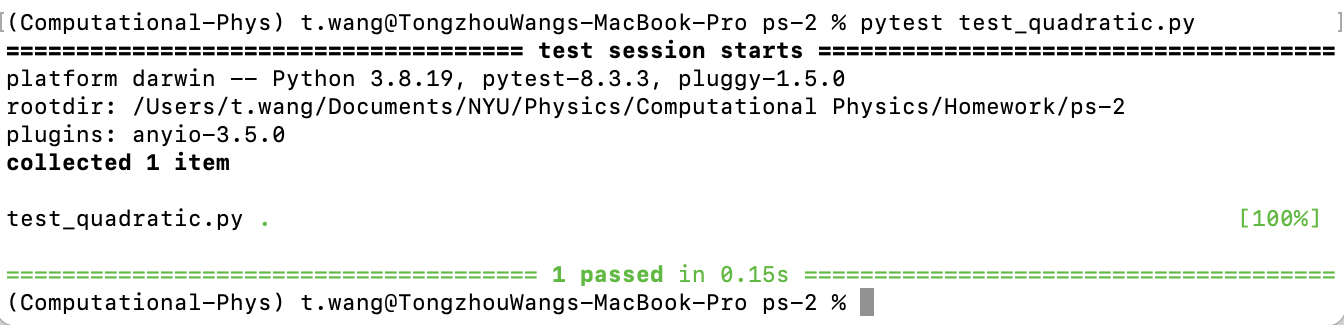
\includegraphics[scale = 0.6]{images/ps-2-5_test-result.png}
    \caption{Unit test result.}
\end{figure}

The function I wrote is shown below. I think the key is to avoid subtractive cancellation errors.

\lstset{style = mystyle}
\begin{lstlisting}[language=Python]
def quadratic(a, b, c):
    v1 = np.abs(np.float64((- b + np.sqrt(np.square(b) - 4 * a * c))))
    v2 = np.abs(np.float64((- b - np.sqrt(np.square(b) - 4 * a * c))))
    
    if v1 > (np.abs(b) / 10):
        x1 = np.float64((- b + np.sqrt(np.square(b) - 4 * a * c)) / (2 * a))
    else:
        x1 = np.float64((2 * c) / (- b - np.sqrt(np.square(b) - 4 * a * c)))
        
    if v2 > (np.abs(b) / 10):
        x2 = np.float64((- b - np.sqrt(np.square(b) - 4 * a * c)) / (2 * a))
    else:
        x2 = np.float64((2 * c) / (- b + np.sqrt(np.square(b) - 4 * a * c)))
        
    return x1, x2
\end{lstlisting}

\end{document}